\part{Clock and Control interface for the Large Pixel Detector} % (fold)
\label{prt:lpd_ccc_interface}

\section{Conventions} % (fold)
\label{sec:conventions}
Throughout this document there are several typographical conventions that are observed (see table~\ref{tab:typography}).

Hexadecimal values are prefaced with `0x' whilst binary values begin `0b' 
% additionally `signal', `lines' and `ports' are used interchangeably to refer to bit(s) of information passed through an interface, either between blocks (e.g.\ from a state-machine to memory) or between cards (e.g.\ between the CCC and FEM). The term `registers' is used to refer to both single (small) blocks of memory and large on-chip block memory (BRAM). Finally a `command word' is a collection of bits that have a specific value and meaning and are presented either serially or in parallel, at an implementation level these are no different from states (which are merely numerical identifiers for the current state) but for clarity these are treated differently i.e.\ command words are transmitted whilst states are internal and not transmitted.
\begin{table}
  \begin{center}
  \begin{tabular}{c|c}
    Type               & Meaning                             \\
    \hline                                                   
    \texttt{lower}     & Port or signal names.               \\
    lower              & Port or signal names (tables only). \\
    CAPS               & Names of generics.                  \\
    \textbf{BOLD CAPS} & Named states of a state-machine.    \\
    \texttt{CAPS}      & Command words.                      \\
  \end{tabular}
  \end{center}
  \caption{Description of typographic conventions.}
  \label{tab:typography}
\end{table}
% section conventions (end)
%%%%%%%%%%%%%%%%%%%%%%%%%%%%%%%%%%%%%%%%%%%%%%%%%%%
\chapter{Introduction} % (fold)
\label{cha:lpd_ccc_introduction}
\section{The European X-ray Free-Electron Laser: an overview} % (fold)
\label{sec:xfel_an_overview}
This is a discussion of the work carried out designing the firmware for the Clock and Control Card (CCC) interface for the Large-Pixel Detector (LPD) at the European X-ray Free-Electron Laser (EuXFEL). There will be a brief discussion of EuXFEL, its aims, the detectors and control systems then a more in-depth look at the design, implementation and testing of the final design.

EuXFEL is a 3.4~km Free-Electron Laser (FEL) being constructed below Hamburg, Germany. The project is scheduled to begin operation in 2016 with commissioning beginning in 2015. EuXFEL is built upon expertise and concepts prototyped at the Free-electron Laser in Hamburg (FLASH) which is operated by DESY although EuXFEL will be operated as an independent research facility. 

Instead of using undulators as merely a method of forcing electrons to emit X-rays (as \(3^{rd}\)~generation synchrotrons do) FELs use much longer undulators to shape the electron beam itself. Micro-bunching is caused as slower electrons absorb the X-rays emitted from faster, following, electrons and faster electrons are slowed as they emit; the result of this is that instead of a single long pulse many small bunches are created that emit light coherently with a much greater brilliance than is seen in synchrotrons.

Production of X-rays at EuXFEL is done by accelerating electrons to 17.5~GeV using a superconducting linear accelerator before passing them through an `undulator' where they produce synchrotron radiation (i.e.\ X-rays). The X-rays at EuXFEL have a wavelength of between 0.05~nm and 4.7~nm, this corresponds to photon energies from 25~keV to 0.26~keV respectively. Each pulse of light will have an average duration of \(\sim\)100~fs and there will be 27,000 flashes per second arranged into 10 `trains', each lasting \(600~\mu\)s. Figure~\ref{fig:xfel-brightness} shows the predicted peak brilliance and energies of X-rays produced at EuXFEL as well as a selection of other existing sources. The divide in brilliances is due to the technology used to power the source, XFEL, FLASH and LCLS all use free electron laser (FEL) system whilst the others are synchrotron sources which gives them a larger range but much lower peak brilliance. 

\begin{figure}[h]
  \centering
    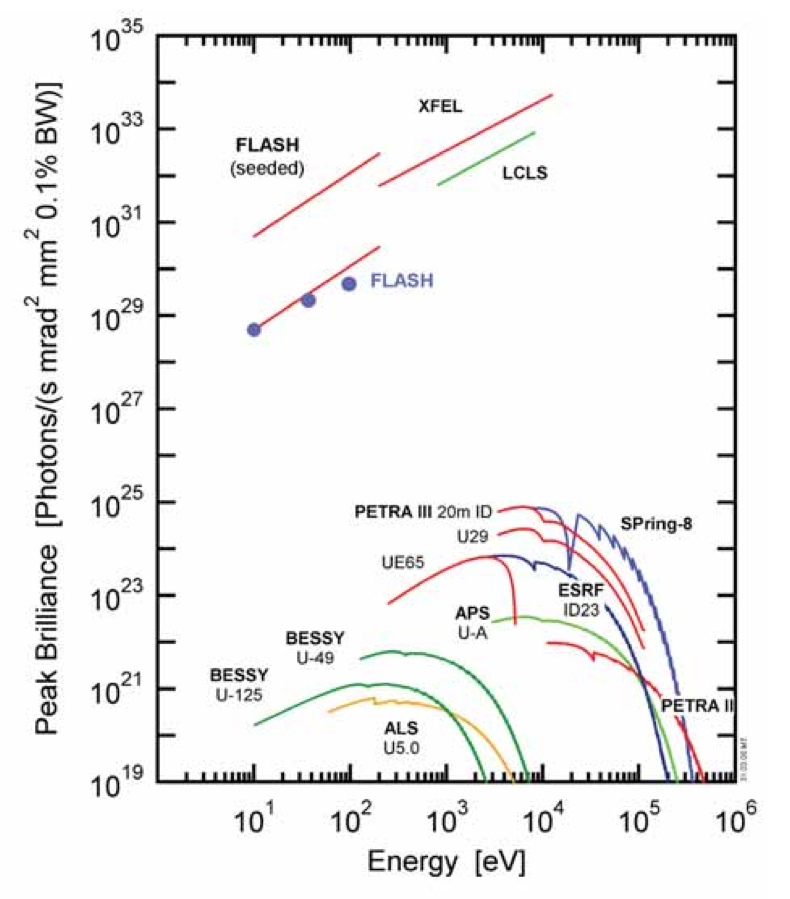
\includegraphics[width=.9\textwidth]{images/Other/XFEL-comparitive_energy-brightness.png}
  \caption{Plot of peak X-ray brilliance against energy for a range of current sources as well as the predicted values for EuXFEL (here labelled `XFEL'). The blue dots show measured peak brilliance for several energies at the existing FLASH facility.}
  \label{fig:xfel-brightness}
\end{figure}

% subsection existing_x_ray_sources (end)
\subsection{Scientific Motivation} % (fold)
\label{sub:scientific_motivation}
The primary aim of EuXFEL is to study conditions previously unseen in a laboratory setting. This aim is achieved through three core properties of EuXFEL: `coherence, ultra-high brilliance and time structure' \cite{CITEATION FOR THE TDR} the combination of these gives access to three broad areas of study: the tiny, the fast and the extreme. In all of these regimes there is much that is unknown or yet to be tested which in turn will lead to new discoveries, new technology and refined techniques.

The imaging of the tiny relies on the wavelength of the light used being comparable to the scale of the structure to be imaged. At EuXFEL as well as having a sufficiently small wavelengths of light (X-rays) to image molecules, due to the coherent nature of the light none-repeating structures can also be imaged. Whilst the brilliance of the beam will destroy most samples very quickly tests at FLASH show that enough time remains to produce a detailed image of the sample, even if it has not been crystallised. This means that larger structures can be imaged at an atomic scale (e.g.\ entire viruses) or structures won't crystallise or only form very small, low quality crystals (e.g.\ protein membranes).

The third of EuXFEL's core properties, time-structure, provides the potential of the second regime, speed. As each individual flash lasts less than \( \sim \)100~fs and each train comprising of 2,700 flashes it's possible to `film' processes as they occur. This will make it possible for researchers to understand what happens during a phase transition or when a material reverses its magnetisation by watching it happen.

The final regime, the extreme, is driven by EuXFEL's brilliance. Able to recreate extreme temperatures and pressures EuXFEL will be able to use `pump and probe' techniques to map, for example: the propagation of shockwaves through a plasma or to image the stresses on a component under extreme magnetic fields.
% subsection scientific_motivation (end)
% section xfel_an_overview (end)
%%%%%%%%%%%%%%%%%%%%%%%%%%%%%%%%%%%%%%%%%%%%%%%  
\section{Detectors at EuXFEL} % (fold)
\label{sub:detectors_at_euxfel}
In order to achieve EuXFEL's scientific program a broad range of detectors are required. For almost all planned experiments there is a need to image the beam's interaction with the target, the standard solution to this is a 2D pixel detector. This type of detector consists of an array of light sensitive pixels, this gives both position and intensity information about the incident light, with minor reconstruction an image of the target can then be formed. The basic requirements for the 2D pixel detectors at EuXFEL are~\cite{xfel_website}:
\begin{description}
    \item[Swiftness] EuXFEL produces 27,000 X-ray pulses per second, ideally all of these need to be recorded.
    \item[Dynamic range] In any one flash the number of photons received by any portion of the detector can vary massively (between 1 and \(10^5\)~\cite{lpd_manual}) this information needs to be preserved by the detector.
    \item[Radiation resistance] When fully operational EuXFEL is intended to be used nearly continuously, obviously any detector used has to be able to survive the harsh environment at the end of the beam-line.
\end{description}

There are currently three 2D pixel detectors being designed for use at XFEL: Adaptive Gain Integrating Pixel Detector (AGIPD), DEPFET Sensor with Signal Compression (DSSC) and Large Pixel Detector (LPD). All three use the above requirements as a base but have employed different technologies in order to meet them.

The main differences between the three detectors are in their implementation of the high dynamic range: LPD and AGIPD both have three different gain levels giving them the required range, whilst DSSC uses the non-linearity of its DEPFET to achieve it. There are a few other significant differences: AGIPD uses dynamic switching to select the appropriate gain; DSSC has hexagonal pixels (AGIPD and LPD have square) and LPD has an entire pipeline for each gain level (this means that when a narrower gain is required it can be set and all three pipelines used for storage). 

\subsection{The Large Pixel Detector (LPD)} % (fold)
\label{sub:the_large_pixel_detector_lpd}
LPD is a 2D, 1~Mega-pixel detector designed at the Rutherford Appleton Laboratory in the UK. The detector is designed to be modular with 1~Megapixel being made up of 16 `supermodules', each supermodule contains a single Front End Module (FEM) that controls and reads out the 128 Application Specific Integrated Circuits (ASICs) that in turn control 512 individual pixels i.e.\ each supermodule is 65,536 pixels divided between 128 ASICs with 1 FEM. It is the FEM that then communicates with the generic elements of EuXFEL: the Clock and Control Card (CCC) and the Train Builder (TB).
    
2 lines are used to control the ASIC during operation: clock (\texttt{clk}) and control (\texttt{cmd}) with a third, slow line being used for configuration. The CCC-interface is responsible for receiving the generic signals from the CCC and converting them to those expected by the ASIC. There are a large number of commands that the ASIC expects in order to function (a full list is given in appendix~\ref{app:asic_command_words}). These commands fall into a a few general groups: starts, (no-)veto\footnote{The ASIC actually uses a `trigger' rather than a `veto', but for consistency with the overall EuXFEL documentation we will use `no-veto' and `veto' to refer to `trigger' and `nop' respectively}, stops, resets, and configuration. In each of these sets of commands there are generally two or tree individual command words that affect a specific component of the ASIC (e.g.\ reset the write pointer, start the trigger pointer). 
    
The FEM that controls the supermodule uses a Xilinx~Virtex-5 FPGA, this has two embedded PowerPC440 processors that manage the resources on the FEM (e.g.\ writing control registers and the dedicated RAM) as well as create the UDP/IP packets that transfer the data from read from the ASIC to the TB. In addition to the CCC-interface there is firmware to organise the read out data from the ASICs, and control configuration. As well as the Virtex-5 there are 2 further Xilinx~Spartan-3's that control fan out of the signals to the individual ASICs.
% subsection the_large_pixel_detector_lpd (end)
% section detectors_at_euxfel (end)
\section{DAQ and control systems} % (fold)
\label{sec:daq_and_control_systems}
In a project the scale of EuXFEL there are a large number of different subsystems that need to communicate flawlessly in order to operate. Not only does a single common clock need to be distributed between all systems but it needs to compensate for the time to transmit a signal between the different components and how this latency may change depending on local conditions (e.g.\ the temperature).

To this end there are several layers of timing and control system used at EuXFEL: top-most is the master oscillator, this is distributed via the timing transmitters to the various systems along with global information about the intended run (e.g.\ the `bunch pattern'). These subsystems must then respond as required to the bunch pattern and any commands received. In addition to globally distributed commands there is also the requirement of intra-system information such as vetoes. 

In the case of the 2D detectors two common control systems were decided upon to act as a common interface to the global timing receivers. The first of these systems is the Clock and Control Card (CCC) which is a client of the timing receiver card that filters commands for its 2D detector clients and distributes a synchronised clock for their use. The second system is the common Train Builder (TB) that acts as a data marshalling card for the various detectors: collating their readout, re-ordering it as required and dispatching it to the batch farm.

\subsection{Clock and Control Card (CCC)} % (fold)
\label{sub:clock_and_control_card}
\begin{figure}[h]
  \centering
    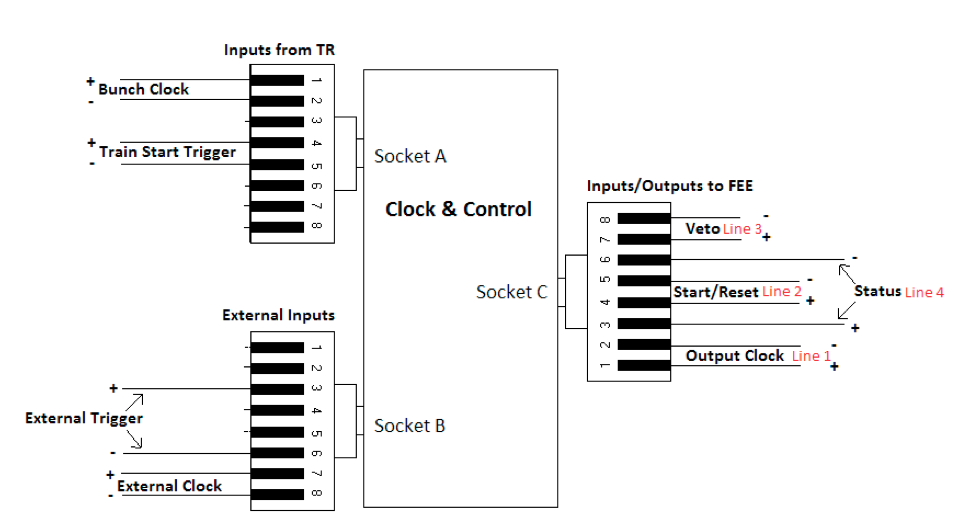
\includegraphics[width=.9\textwidth]{appendix_XFEL/images/Other/CCC_RJ45_diagram.png}
  \caption{The CCC RJ45 wiring diagram.}
  \label{fig:CCC_RJ45_diagram}
\end{figure}

As discussed above the CCC is one of two cards common to all 2D detectors, it has four primary functions in EuXFEL: distribution of the clocks required to maintain synchronicity with the rest of the machine, signalling of veto information for each bunch, control of the attached FEMS and collection of status information. In addition to these requirements it can also operate in standalone mode (detached from a TR board) in order to facilitate testing and for use at other locations (e.g.\ LCLS). 

The CCC communicates with any attached FEMs via RJ45 (see figure~\ref{fig:CCC_RJ45_diagram}), the four paired wires carry the four signals as required: clock, fast-command, veto and status. The clock signal is 99~MHz derived from the TR, the fast command line carries information about each train whilst the veto line carries information on whether a bunch should be kept, the status line returns the received clock to indicate correct connections. Each of these lines (with the exception of the status) are discussed below.

% subsection clock_and_control_card (end)
\subsubsection{Clock signal} % (fold)
\label{sub:clock_signal}
\begin{figure}[h]
  \centering
    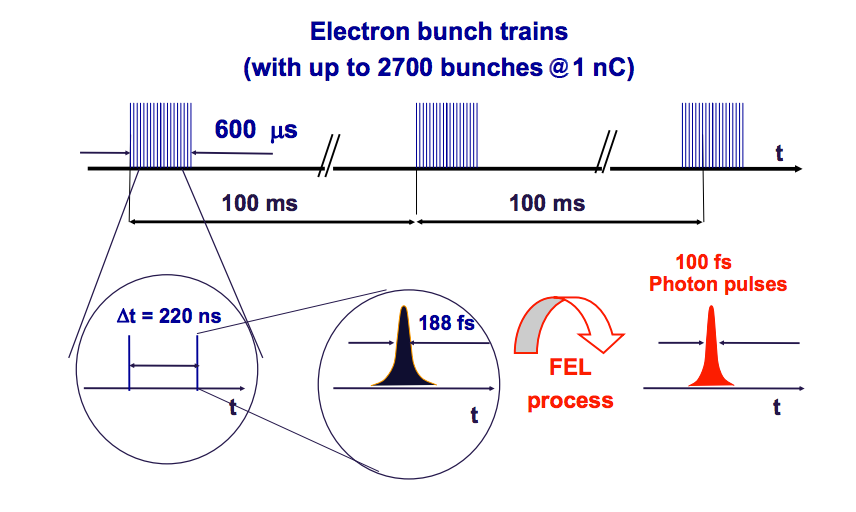
\includegraphics[width=.9\textwidth]{appendix_XFEL/images/Other/XFEL-time_structure.png}
  \caption{The timing structure of electrons at EuXFEL and the resultant X-ray pulses. }
  \label{fig:XFEL-time_structure}
\end{figure}

An interesting aspect of EuXFEL is its timing structure, rather than a simple monoatomic pulse it has two regular bunch trains containing several thousand pulses (or `bunches') each. The trains arrive at a rate of 10~Hz with each lasting only 600~\(\mu\)s but containing up to 2,700 100~fs bunches each separated from the next by \( \sim \)220~ns figure~\ref{fig:XFEL-time_structure} shows this.

This timing structure forces the detectors to use the time between bunches for data readout while during the bunch train they are limited to just storing data. This means that each detector is limited by the length of its on-ASIC pipeline with regards to how much data it can store (for LPD this is either 512 frames if using all three gain levels or 1536 if only using one). This structure also means there are two cycles that the detectors need to be aware of: firstly the bunch clock (\(\sim\)4.5~MHz) and secondly the bunch-train clock (\(\sim\)10~Hz). Finally, in addition to these two machine imposed clocks there is the common CCC fast clock that is used for transmitting commands from the CCC which has a frequency of \(\sim\)99~MHz.
% subsection clock_signal (end)
\subsubsection{Control signal} % (fold)
\label{sub:control_signal}
The control signal is used to convey information about the train. This information comes in four parts: when the next train will start, when it will stop, which train it is (its ID) and what bunch pattern applies (see section~\ref{sub:veto_signal}, below). There is also a reset command to indicate that the ASIC and FEM should be reset to a known state. 

The start signal is assumed to arrive, with some fixed latency, ahead of the first bunch in the train. The stop signal is similarly assumed to have some fixed latency from the last. In addition to warning of the beginning of the train the start signal also has an attached payload of information about the train: the train ID and the bunch pattern. The specification for these signals is given in table
\begin{table}
  \begin{center}
  \begin{tabular}{c | c | c | c}
    Command  & Bits   & Payload & Description \\
    \hline   
    START    & 0b1100 & Train ID (32b), bunch pattern ID (8b), checksum (8b) & Start of the train \\
    STOP     & 0b1010 & none                                                 & End of the train \\
    RESET    & 0b1001 & none                                                 & Reset the FEM and ASIC \\
    reserved & 0b1111 & n/a                                                  & n/a\\
  \end{tabular}
  \end{center}
  \caption{Specification of the fast command signals and their payloads.}
  \label{tab:fast_commands}
\end{table}
% subsubsection control_signal (end)
\subsubsection{Veto signals} % (fold)
\label{sub:veto_signal}
Given the previous discussion of the 2D detectors at EuXFEL (section~\ref{sub:detectors_at_euxfel}) it is obvious that it is impossible for them to record all 2.700 bunches of the data, equally with a single linac being divided between five, and later ten, experimental stations not every detector will be receiving all of the bunches for every train. To account for this there are two veto systems that allow the detectors to select which bunches they should record for processing: the `bunch pattern' and the online veto. Either of these two sources may veto a bunch so it is only recorded if neither source vetoes it. 

The bunch pattern veto (although it is more of a trigger) is derived from the global configuration of the machine: if, for example, the first half of the electron beam is being sent to another experimental station the detector will receive a pattern that tells it to veto that portion of the train. The patterns act as masks: for each bunch in a train the pattern states whether it should be vetoed or not. The bunch patterns are decided ahead of time, and loaded when the FEM is configured the bunch pattern to be used for each train is signalled prior to its arrival as part of the start signal sent via the command line.

The online vetoes are mainly situational, if the beam doesn't lase or there is an fault there is rarely any point taking data, in which case those bunches should be vetoed. These online vetoes can have any source and the signals are supplied to a dedicated veto unit that is external to the CCC. The CCC will in turn pass on the veto or no-veto signal to the FEM of the detector, either with an attached bunch ID or with a fixed latency from the bunch in question depending on the specifications of the detector. There is an additional `golden' mode that selects bunches that should be preferentially kept giving three levels of selection: dispose, keep if possible and keep although this is not implemented for LPD. It is these veto signals that are received via the veto line as well as the bunch ID (which LPD ignores) the structure of these signals is given in table~\ref{tab:veto_spec}.

\begin{table}
  \begin{center}
  \begin{tabular}{c|c|c|c}
    Command & Bits   & Payload                        & Notes\\
    \hline
    VETO    & 0b110  & \multirow{2}{*}{Bunch ID (8b)} & Veto this bunch \\
    NOVETO  & 0b101  &                                & Record this bunch \\
    reserved& 0b111  & n/a                            & n/a \\
  \end{tabular}
  \end{center}
  \caption{Veto signal specification}
  \label{tab:veto_spec}
\end{table}
% subsection the_clock_and_control_card_ccc (end)
%%%%%%%%%%%%%%%%%%%%%%%%%%%%%%%%%%%%%%%%%%%%%%%
% section daq_and_control_systems (end)
\section{Firmware} % (fold)
\label{sec:firmware}
Firmware describes a broad range of technologies that bridge the divide between hardware (the physical chip and wires) and software (a program intended to run on a generic processor). Whilst firmware can refer to anything as complex as a set of embedded programs run on a piece of hardware in this document it is used to refer to the specific logic loaded onto a programmable chip to configure its operation.

The LPD firmware is run on Field Programmable Gate Arrays (FPGA) which combine logic `slices' and on board memory to create flexible and powerful chips. This means that software can be used to control configuration settings for the firmware which then can run with very low latencies and in a highly predictable manner. A key property of an FPGA is that when it loads its firmware it physically changes its configuration to implement the logic described. It's important to note that most modern FPGAs can also implement processors (called `softcores') that can run custom programs as well, for LPD this ability is used to simplify configuration of the FEM.

\subsection{VHDL} % (fold)
\label{sub:vhdl}
There are a variety of languages for writing firmware, the one used for LPD is VHSIC\footnote{Very High Speed Integrated Circuit} Hardware description language (VHDL). VHDL works by describing the expected operation of various discrete blocks within the firmware, these descriptions are then translated (synthesised or compiled) into bit-code that, in the case of FPGAs will tell the chip how to configure its slices.

Whilst a detailed description of the language are beyond the scope of this document there are several attributes of it that are required to understand the following discussions. The first major feature of VHDL to be understood is that it is a \emph{description} language as such the specification makes few guarantees about how any particular block of logic will be implemented as the it only defines what the syntax means, the same code may produce very different results depending on the synthesiser used and the chip being targeted.\footnote{Assuming that the code isn't being used to produce an ASIC.}

As discussed above the chips being used to implement the FEM firmware are FPGAs that consist of `slices', the general layout of these slices is logic then a Look Up Table (LUT). This logic/LUT means that many designs are resolved to `apply logic to signals' then `look up value of signals in table' finally `out put value stored in table'. The result of this system is that most designs are split into two groups of components the `state-machine' and the `memory'. A state-machine is a set of states with attached conditions, the inputs to the state-machine determine which state should be selected and then that state determines what the output should be, the memory stores any persistent information needed by the state-machine either as input, or output.

In VHDL blocks of code (`entities') are defined by their ports and generics. Ports represent in or out-bound signals\footnote{VHDL also specifies `inout' as a bi-directional port but they are not used here.} these can either be single or grouped into vectors. The generics associated with an entity define values that may need to change on a per-synthesisation time-frame, they're mainly used in the design to specify useful defaults for registers and values that shouldn't be changeable at run time but may need to change between systems (e.g.\ delays). An entity is specified by its ports, generics and its name, a single entity can have multiple implementations (different `architectures') but this capability is not used here.

VHDL specifies two broad classes of value that can be used for ports: signals and vectors, a signal is a single bit of information whilst a vector is a collection of bits in some order. VHDL's basic type of signal is called `std\_logic' (sl). Sl is generally used for transfer of the boolean values (`1' or `0'), it can take several other values (`L', `H', `U', `W', `X', `Z' and `-') that specify hardware signals (e.g.\ `L' specifies a weak signal that should probably be low). The vector form of sl is a `std\_logic\_vector' (slv) that is ordered `X to Y' or `Y downto X', if the slv is converted to a numeric type (e.g.\ an integer) then this ordering determines the `endedness'. E.g.\ if an slv (3 downto 0) is 0b1000 then its integer value is 8, the same value (0b1000) but with ordered reversed (i.e.\ 3 to 0) as an integer is 1. Through out this document order is denoted using parenthesis e.g.\ slv~(3:0) is a std\_logic\_vector~(3~downto~0) while slv~(0:3) is (3~to~0). In addition to the std\_logic types VHDL does implement numeric types (`signed', `unsigned' and `integer') but these aren't used at top level interfaces as they can cause synthesis problems.
% subsection vhdl (end)
%%%%%%%%%%%%%%%%%%%%%%%%%%%%%%%%%%%%%%%%%%%%%%%%%%%
% section firmware (end)
%%%%%%%%%%%%%%%%%%%%%%%%%%%%%%%%%%%%%%%%%%%%%%%
